\documentclass[letter,10pt]{article}
\usepackage[utf8]{inputenc}
\usepackage{graphicx}
\usepackage{natbib}
\usepackage{hyperref}
\usepackage{courier}
\usepackage[margin=0.75in]{geometry}
\usepackage[table,svgnames]{xcolor}
\usepackage{multirow}
\usepackage{tabu}
\usepackage{float}
\usepackage{listings}
\usepackage{xspace} 
\bibliographystyle{unsrtnat}
\definecolor{HeaderColor}{rgb}{0.8, 0.8, 0.95}
\setlength{\parindent}{0pt}
\setlength{\parskip}{6pt}

\usepackage[T1]{fontenc}
\usepackage[utf8]{inputenc}
\usepackage{authblk}

\author[1,2]{Dimitri Yatsenko\thanks{dvyatsen@bcm.edu}}
\affil[1]{Department of Neuroscience, Baylor College of Medicine, Houston, Texas, USA}
\affil[2]{Vathes LLC, Houston, Texas, USA}

\renewcommand\Authands{ and }
\newcommand{\datajoint}{DataJoint\xspace}


\graphicspath{{./figures/}}

\lstset{
    backgroundcolor=\color{white},
    tabsize=4,
    basicstyle=\ttfamily,
    breaklines=true
    framextopmargin=50pt,
    aboveskip={0.5\baselineskip},
    columns=fixed,
    frame=single,
    showstringspaces=false,
    extendedchars=false,
    breaklines=true,
    numbers=none,
    showtabs=false,
    showspaces=false,
    showstringspaces=false,
    identifierstyle=\color[rgb]{0.0,0.2,0.0},
    keywordstyle=\bfseries\color[rgb]{0.2,0.2,0.6},
    commentstyle=\color[rgb]{0.4,0.6,0.6},
    stringstyle=\color[rgb]{0.6,0.0,0.2},
    numberstyle=\tiny\color[rgb]{0.6, 0.6, 0.6}}

\lstdefinelanguage{dj}{
  keywords={int, smallint, char, varchar, enum, unsigned, date, year, decimal},
  keywordstyle=\color{blue},
  keywords=[2]{boolean, string, number, objectid},
  keywordstyle=[2]\color{green}\bfseries,
  identifierstyle=\color{black},
  sensitive=true,
  morecomment=[l][\color{teal}\bfseries]{::},
  morecomment=[l][\color{gray}\itshape\small]{\#},
  stringstyle=\color{red},
  morestring=[b]',
  morestring=[b]"
}

\newfloat{lstfloat}{htbp}{lop}
\floatname{lstfloat}{Listing}

\title{\datajoint: A Simpler Relational Data Model and Language}

\begin{document}

\maketitle
\begin{abstract}
A simplified and conceptually refined relational data model is proposed with a language for schema definition and data queries as well as a diagramming method for visualizing relationships among the data.  
Named \datajoint, the model adheres to the principle of \emph{operational entity integrity}, which requires that all data --- both stored and derived --- exist in the form of sets of entities belonging to well-defined entity classes.  
\datajoint's data query language is an algebra of five operators that provide equal capabilities to those of other relational query languages with greater clarity due to adherence to operational entity integrity. 
Practical implementations of \datajoint known as DataJoint haves been tested and adopted for scientific data pipelines.  
With \datajoint, programmers interact with scientific data more fluently than with other data definition and query languages.
\end{abstract}
\tableofcontents 

\twocolumn

\section{Core Concepts}
\subsection{The Relational Data Model}
The relational data model \citep{codd_relational_1970} provides the most rigorous approach to structuring stored data as well as the most precise approach to querying stored data.  
Briefly, the relational data model is characterized by the principles of data representation, domain constraints, uniqueness constraints, referential constraints, and declarative queries as summarised in Table \ref{tab:core}.

\tabulinesep=6pt
\begin{table*}[ht]
\begin{tabu}{|X|}
\hline
{\bf Data representation.} Data are represented and manipulated in the form of \emph{relations}. 
A relation is a set (unordered collections) of \emph{tuples} of values for each of the respective named \emph{attributes} of the relation.
\emph{Base relations} represent stored data while \emph{derived relations} are formed from base relations as a result of data queries.
A collection of base relations with their attributes, domain constraints, uniqueness constraints, and referential constraints is called a \emph{schema}.

\\
{\bf Domain constraint.} Attribute values are drawn from corresponding attribute \emph{domains}, \emph{i.e.}\ predefined sets of values.
Attribute domains may not include other relations, ensuring that the relational model is essentially flat with no nesting data structures.

\\
{\bf Uniqueness constraints.} Tuples within relations are addressed by values of their attributes.
To identify and relate data elements, \emph{uniqueness constraints} on a subset of attributes may be imposed so that no two tuples can have the same values of these attributes.  The set of attributes with a uniqueness constraints are referred to as a \emph{key}. One in a relation key may be designated as the \emph{primary key} for the relation to serve for referencing elements in a relation.

\\
{\bf Referential constraints.} Associations among data are established by means of \emph{referential constraints} in the form of \emph{foreign keys}. 
Referential constraints prohibit tuples in one relation that lack tuples with matching values in the referenced relation. 

\\
{\bf Declarative queries.} \emph{Query expressions} produce derived relations from base relations.  
Query expressions declare specifications for retrieving data rather than a procedural one. 
Formal languages for query expressions include \emph{relational algebra} and \emph{relational calculus}.  
\\
\hline
\end{tabu}
\caption{Core principles of the relational data model.}
\label{tab:core}
\end{table*}

Popular implementations of the relational data model rely on the Structured Query Language (SQL) for schema definition, data manipulation, and data queries.
SQL so thoroughly dominates in the space of relational databases that it has become nearly synonymous with the relational data model despite notable deviations from its core principles.

\datajoint is a clean, conceptually refined implementation of the relational data model adhering faithfully to its core principles.
Its introduction is motivated by the need for expressive and flexible conceptual and logical constructs for database programming in scientific computing.

\datajoint comprises 
\begin{itemize}
\item a \emph{schema definition language} (Sections \ref{sec:def1} and \ref{sec:def2}),
\item a \emph{data manipulation language} (Section \ref{sec:manip}),
\item a \emph{data query language} (Section \ref{sec:query}), and 
\item diagramming notation for visualizing relationships between modeled entities (Section \ref{sec:diag}). 
\end{itemize}

\subsection{Conceptual Clarification}
The relational model in itself is abstract and semantically unconstrained, providing few guidelines for translating real-world entities and relationships into database schemas or for forming valid queries. 
For schema design, a set of formal rules known as \emph{normal forms} has been defined to test whether a particular schema meets basics quality requirements that minimize redundancies in data storage and anomalies in data manipulations \citep{kent-1983-simple}.
For data queries, the relational data model provides few constraints as to what constitutes a valid or meaningful query, allowing unlimited freedom to compare and match different relations and attributes regardless of their semantic compatibility.
This lack of conceptual clarity has led to a diversity of incompatible approaches to schema design and data queries, slow learning, and limits on complexity of schemas designs and data queries.

To address these problems and to bring conceptual clarity to database schema design and data queries, Peter Chen proposed a new variant of the relational data model known as the Entity-Relationship Model (ERM) \citep{chen_entity_1976}.
In the ERM, each base relation denotes either an \emph{entity set} or a \emph{relationship set} and these terms effectively subsume the term \emph{relation}.

Table \ref{tab:terms} correlates the terms used by each variant of the relational data model. 

All elements of a given entity set must belong to the same \emph{entity type} with the same set of attributes and distinguished from each other by the same primary key attributes.

Each entity set may only contain entities of the same class, sharing the same set of attributes and distinguished by the same  primary key.
Foreign keys between relationship sets and entity sets express and enforce the corresponding relationship.

In ERM, query expressions follow patterns established through relationship sets between entity sets, providing a correspondence between the schema design and sensible queries. 
The development of ERM stopped short of defining a formal query language distinct from those of the broader relational model.

Despite its origin as a relational data model in its own right, ERM is now taught as an abstract model for \emph{conceptual modeling} with expressive diagramming notation.  
Modern introductory texts and courses on relational databases distinguish \emph{conceptual modeling} from \emph{logical design} as separate phases of database design and implementation \citep{elmasri-2015-fundamentals, coronel-2016-database}.
SQL does not explicitly embody ERM, practicing programmers internalize its concepts and  mentally or explicitly categorize tables as either ``entity tables'' or ``relationship tables''.  
ERM designs tend to produce database schemas that already  meet rules of database normalization from formal relational database theory and practicing database developers rarely need to recall the definitions of normal forms from their formal academic training.

\subsection{Entity integrity}
In the ERM, an entity is defined as distinct and identifiable within its entity set. 

In database theory, the \emph{entity integrity} constraint is the requirement that relations must have an explicit primary key and that values of the primary key attributes cannot be missing (null). 

In this paper, we use the term \emph{entity integrity} more broadly as the property of a relational database to respect its relations as entity sets.

Different variants of the relational data model use different terminology to refer to similar concepts (Table \ref{tab:terms}).
\tabulinesep=6pt
\begin{table*}[ht]
   \rowcolors{1}{white}{gray!20}
   \begin{tabu}{|X[1,c,p]| X[1,c]| X[1,c]| X[1,c]|}
   \hline
   \rowcolor{HeaderColor}
   {\bf Relational} & {\bf ERM} & {\bf SQL} & {\bf \datajoint}  \\
   \cellcolor{white} & entity set & \cellcolor{white} & \cellcolor{white} \\
   \multirow{-2}{*}{relation}  & relationship set  & \multirow{-2}{*}{table}  &  \multirow{-2}{*}{entity set} \\
   tuple       & entity           & row    & entity \\
   domain      & value set        & data type & data type \\
   attribute   & attribute        & column {\em or} field    & attribute \\
   attribute value & attribute value  & field value & attribute value \\
   primary key & primary key & primary key & primary key \\
   foreign key & foreign key & foreign key & foreign key \\
   schema      & schema      &  schema  &  schema \\
   relational expression \par {\em or} derived relation &  data query & {\tt SELECT} statement & query expression \\
   \hline
   \end{tabu}
\caption{Corresponding terms used in variants of relational models.}
\label{tab:terms}
\end{table*}

\datajoint provides a simpler, conceptually refined relational data model that is as expressive as it is practical. 
These conceptual refinements eliminate the gap between conceptual modeling and logical design in database development.

Fundamentally, \datajoint is a relational data model.  This means that its basic and only data structure is a \emph{relation}.
Additionally, every relation represents an \emph{entity set}: an unordered collection of identifiable items in the modeled world that have the same set of attributes, are distinguished from each other by the same \emph{primary key}, and participating in the same kinds of dependency relationships  with other entity sets. 
Secondary attribute values may be omitted in some elements of an entity set (\emph{i.e.}\ set to null. 
However,  primary key attributes of any element of an entity set cannot be null. 

\datajoint's definition of an entity set is essentially equivalent to that used in the ERM.
Relations and entity sets are often visualized in the form of \emph{tables}. 
Therefore, in \datajoint the terms \emph{relation}, \emph{entity set}, and \emph{table} can be used interchangeably even though this equivalence does not generally hold in other data models. 
Individual elements of an entity set may be called \emph{entity instances}, \emph{tuples}, or \emph{rows}.
The attributes of an entity set may also be called \emph{columns} or \emph{fields}. (See Table \ref{tab:terms}).


\begin{description}
\item[The schema definition language] allows defining the structure of the stored entity sets (base entity sets)  and their interdependencies.  
\item[The data manipulation language] allows updating the stored data.
\item[The data query language] allows deriving entity sets (\emph{derived entity sets}) from base entity sets using \emph{relational expressions}.
\end{description}

All three sublanguages respect the definition of relations as entity sets.  
In particular,  data resulting from queries appear as well-formed entity sets with a clearly expressed entity type, primary key. 
We refer to this innovation as \emph{operational entity integrity}. 

Operational entity integrity is related to the concept \emph{entity integrity constraint} in conventional database systems but applies to derived data as well as stored data.

\section{Schema Definition --- Basics.}\label{sec:def1}
\datajoint's  \emph{schema definition language} allows defining base entity sets and dependencies between them. 

\subsection{Entity-set declaration}
A schema is defined by declaring a collection of \emph{base entity sets}.
An entity set is a set of distinct and identifiable entities from the model world. 
A base entity has a unique name within the schema 

\begin{lstfloat*}
\begin{lstlisting}[language=dj]
::Student     
student_id : int unsigned   # university-wide ID number 
---
first_name      : varchar(40)
last_name       : varchar(40)
sex             : enum('F', 'M', 'U')
date_of_birth   : date
student_address : varchar(200) # mailing address
student_phone   : varchar(14) 

::Department 
dept : varchar(6)   # abbreviated department name, e.g. BIOL
---
dept_name    : varchar(200)  # full department name
dept_address : varchar(200)  # mailing address
dept_phone   : varchar(14)  

::StudentMajor
-> Student
---
-> Department
declare_date :  date  # when student declared her major  
\end{lstlisting}
\caption{University database schema definition (Part 1).}
\label{lst:uni1}
\end{lstfloat*}

\begin{lstfloat*}
\begin{lstlisting}[language=dj]
::Course     
-> Department
course  : int unsigned   # course number, e.g. 1010
---
course_name :  varchar(200)  # e.g. "Neurobiology of Sensation and Movement."
credits     :  decimal(3,1)  # number of credits earned by completing the course

::Term
term_year : year 
term      : enum('Spring', 'Summer', 'Fall')

::Section 
-> Course
-> Term 
section : char(1)
---
auditorium   :  varchar(12)

::CurrentTerm
---
-> Term

::Enroll
-> Section
-> Student 

::LetterGrade
grade : char(2)
---
points : decimal(3,2)

::Grade 
-> Enroll
---
-> LetterGrade

\end{lstlisting}
\caption{University database schema definition (Part 2).}
\label{lst:uni2}
\end{lstfloat*}

\begin{figure}
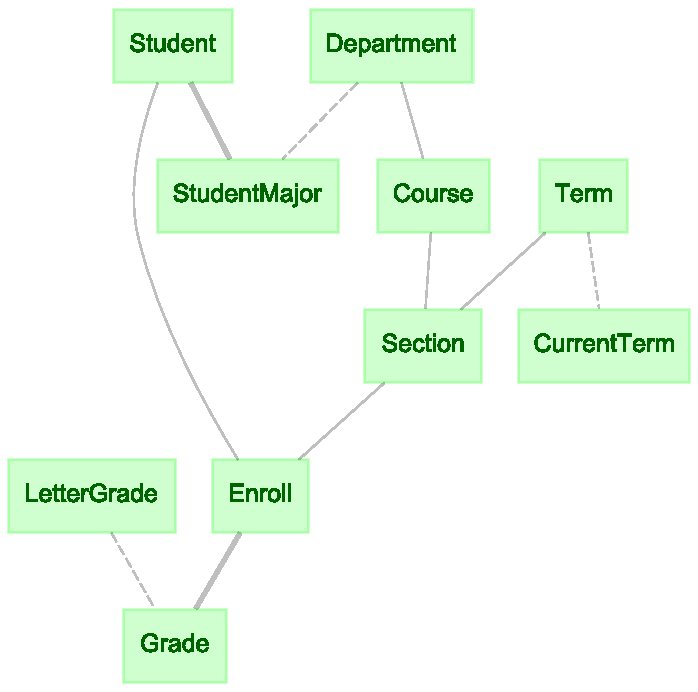
\includegraphics[width=\columnwidth]{uni_erd.pdf}
\caption{The schema diagram of the university database.}
\label{fig:erd}
\end{figure}


\subsubsection{Attributes and their datatypes}
\subsubsection{Primary key}

\subsection{Dependencies}
\subsubsection{Effects of dependencies}
\subsubsection{Primary and secondary dependencies}
\subsubsection{Acyclicity}

\subsection{Schema diagrams}\label{sec:diag}

\section{Data manipulation}\label{sec:manip}
\subsection{Insert}
\subsection{Delete}
\subsection{Cautious update}

\section{Query Expressions}\label{sec:query}
\subsection{Relational operators and expressions}
\subsection{Operational entity integrity}
\subsection{Join compatibility}
\subsection{Restriction}
\subsubsection{Restriction by attribute conditions}
\subsubsection{Restriction by other relations}
\subsubsection{Restriction by a list}

\subsection{Join}
\subsection{Projection}
\subsection{Union}
\subsection{Aggregation}
Aggregation functions cannot be used in restrictions. 
\subsection{Relation U}

\section{Schema Definition --- Advanced.}\label{sec:def2}
\subsection{Dependencies on query expressions}
\subsection{Master-part relationship}
The primary motivation for the master-part relationship is to inform the application that the master and all its parts should always appear together or not at all.  
This usually means using transactions.  
A transaction starts then the master is inserted, then all the parts, and only then the transaction is committed.  
This way all other users only see the master entry when all its parts have been entered.
A part may be in 1-to-1 relationship with its master without any new primary attributes.
\subsection{Dependency properties}

\section{Discussion}
The relational model for databases has been around for nearly fifty years and its use has been standardized by a wide adoption of SQL.
However, some lack of conceptual clarity of SQL and the relational data model make them unwieldy for conceptual design and complex queries. 
As a result, the field has converged on the understanding that database design consists of two distinct components: \emph{conceptual modeling} and \emph{logical modeling} leading to physical implementation. 
Although the Entity Relationship Model was proposed as a model suitable for both conceptual modeling and definition of database schemas, it never replaced the refined data definition languages and evolved into a tool limited to conceptual modeling.  
Furthermore, the ERM's conceptual clarifications chiefly pertain to schema definition and do not provide a data query language with the same level conceptual clarification for derived results as for stored data.

The relational data model and its query languages relational algebra and relational calculus are not concerned with observing. 

SQL in term is implemented to support the general unrefined relational data model while also deviating from it in significant ways. 
Although most SQL programmers 



\appendix

\section{Differences from SQL}
Faithful adherence to the relational data model. 
Native entity integrity.

\subsection{SQL Translations}


\bibliography{DataJoint}

\end{document}
